% f2015zjl_q19_ellipse.tex — 2015 年高考数学·浙江卷·理科 第 19 题（椭圆与对称弦）
%
% 【来源】`.work/phase3-b19/source/2015浙江理.pdf`（SHA-256
%   801150f0a6d440ac967813d264face6d48b6ee9c69cc20f1c9d6b2b38dec2e9f），
%   第 2 页（合订本页 990）；内容对象 23。逐路径实测见
%   `.work/phase3-b19/figure-inventory.md`。
%
% 【坐标口径】源 PDF 用户空间（原点左下、y 向上）。本图本地坐标
%   (x, y) = (x_page − 599.627, y_page − 586.119)，1 单位 = 1 TeX pt。
%   路径坐标逐点照录内容流（含三次贝塞尔控制点）。
%
% 元素计数：9 条路径（x/y 轴＋箭头、椭圆、对称轴、OA/OB/AB）＋5 个标签
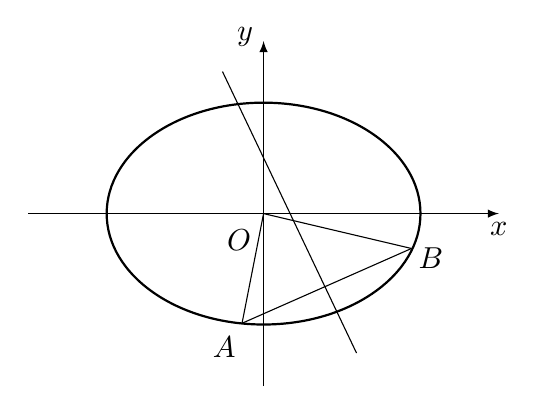
\begin{tikzpicture}[x=1pt, y=1pt,
    every node/.style={inner sep=0pt, font=\fontsize{10.5pt}{12.6pt}\selectfont}]
  \draw[line width=0.3985pt] (-0.0004,62.3630)   -- (166.4939,62.3630);
  \fill[line width=0.3985pt] (170.0804,62.3630)   .. controls (169.0177,62.5622) and (167.2909,63.1600) .. (166.0954,63.8574)   -- (166.0954,60.8686)   .. controls (167.2909,61.5660) and (169.0177,62.1637) .. (170.0804,62.3630);
  \draw[line width=0.3985pt] (85.0400,0.0001)   -- (85.0400,121.1393);
  \fill[line width=0.3985pt] (85.0400,124.7259)   .. controls (84.8408,123.6632) and (84.2430,121.9363) .. (83.5456,120.7408)   -- (86.5344,120.7408)   .. controls (85.8370,121.9363) and (85.2393,123.6632) .. (85.0400,124.7259);
  \draw[line width=0.79701pt] (85.0400,62.3630)   (141.7336,62.3630)   .. controls (141.7336,84.5002) and (116.3514,102.4454) .. (85.0400,102.4454)   .. controls (53.7286,102.4454) and (28.3464,84.5002) .. (28.3464,62.3630)   .. controls (28.3464,40.2258) and (53.7286,22.2806) .. (85.0400,22.2806)   .. controls (116.3514,22.2806) and (141.7336,40.2258) .. (141.7336,62.3630)   -- cycle   (85.0400,62.3630);
  \draw[line width=0.3985pt] (85.0400,62.3630)   -- (138.4822,49.7545);
  \draw[line width=0.3985pt] (85.0400,62.3630)   -- (77.2617,22.7287);
  \draw[line width=0.3985pt] (118.6253,11.9736)   -- (70.1862,113.6905);
  \draw[line width=0.3985pt] (77.2617,22.7287)   -- (138.4822,49.7545);

  \node[anchor=center] at (78.373,126.121) {$y$};  % 源中心 (678.00,712.24)
  \node[anchor=center] at (76.173,52.721) {$O$};  % 源中心 (675.80,638.84)
  \node[anchor=center] at (70.873,13.921) {$A$};  % 源中心 (670.50,600.04)
  \node[anchor=center] at (170.073,56.771) {$x$};  % 源中心 (769.70,642.89)
  \node[anchor=center] at (145.473,46.371) {$B$};  % 源中心 (745.10,632.49)

\end{tikzpicture}
%
% 【自验结果】
%   探针：latexmk -pdfxe（待跑）。
